\documentclass[11pt,a4paper]{article}
\usepackage[margin=2.2cm]{geometry}
\usepackage{booktabs,graphicx,listings,xcolor,amsmath,hyperref,float,enumitem}
\hypersetup{colorlinks=true,linkcolor=blue!50!black,urlcolor=blue!50!black}
\lstset{basicstyle=\ttfamily\footnotesize,breaklines=true,frame=single,backgroundcolor=\color{gray!6},columns=fullflexible}
\begin{document}
\maketitle
\tableofcontents
\newpage

\section{Problem and approach}
The 8-puzzle is a $3\times3$ board with tiles $1\ldots8$ and a blank (written $0$). A \emph{state} is a tuple of nine integers read row by row, e.g. \texttt{(1,2,5,3,4,0,6,7,8)}. The \emph{goal} is \texttt{(0,1,2,3,4,5,6,7,8)}. The four actions \texttt{Up, Down, Left, Right} move the \textbf{blank} one cell; each action costs 1, so the path cost equals the number of moves.

I implemented the four required algorithms --- BFS, DFS, Iterative-Deepening DFS (IDS) and A* --- and A* with two heuristics (Manhattan and Euclidean). Everything is written in Python 3 with the standard library only.

\subsection{Assumptions and details}
\begin{itemize}[nosep]
\item Only half of the $9!$ boards are solvable. A board is solvable iff the number of inversions (ignoring the blank) is even; the program checks this first and refuses unsolvable input (\texttt{is\_solvable}).
\item Children are generated in the fixed order Up, Down, Left, Right, so every run is deterministic.
\item \textbf{Counting rule (identical for all algorithms).} \emph{Nodes expanded} increases by one each time a node is taken from the frontier, is not the goal, and its children are generated. The goal test happens when a node is \emph{removed} from the frontier. \emph{Search depth} is the depth of the goal node; \emph{cost} is the length of the returned path; \emph{running time} is wall-clock time measured with \texttt{time.perf\_counter()} around the search only.
\item DFS and BFS use a visited set (graph search) so they terminate. IDS cannot use a global visited set (see \S\ref{sec:ids}).
\end{itemize}

\subsection{Code structure}
\begin{tabular}{@{}ll@{}}
\texttt{puzzle/state.py} & state representation, neighbours, solvability, random states\\
\texttt{puzzle/result.py} & \texttt{SearchResult} record and path reconstruction\\
\texttt{puzzle/bfs.py, dfs.py} & breadth-first and depth-first search\\
\texttt{puzzle/ids.py} & \textbf{iterative deepening DFS (new)}\\
\texttt{puzzle/astar.py} & \textbf{A*, Manhattan and Euclidean heuristics (new)}\\
\texttt{puzzle/visualize.py} & traceable text output (every step printed as a board)\\
\texttt{main.py} & command-line driver, timing, comparison table\\
\texttt{gui.py} & \textbf{graphical interface (new)}\\
\texttt{tests/test\_algorithms.py} & 24 automated tests
\end{tabular}

\section{Algorithms}
\subsection{Breadth-first search}
BFS expands nodes level by level using a FIFO \texttt{deque}; a \texttt{visited} set avoids repeats and a \texttt{parents} dictionary \texttt{\{state: (parent, move)\}} rebuilds the path. With unit costs, the first time the goal is reached is at the minimum depth, so BFS is \emph{complete and optimal}. Cost: $O(b^d)$ time \emph{and} memory, which is its weakness (179{,}170 expansions for a 28-move board).

\subsection{Depth-first search}
DFS uses a LIFO stack (a Python list) and a visited set. It dives down one branch before trying the next. It is complete here only because of the visited set, but it is \emph{not optimal}: it returns the first solution it meets, which is usually enormously long (see the DFS rows in the results: 31 moves for a 3-move puzzle, 86{,}930 moves for seed 7).

\subsection{Iterative-deepening DFS (IDS)}\label{sec:ids}
\textbf{Idea.} Run a depth-limited DFS with limit $0,1,2,\dots$ until the goal is found. Memory is only $O(d)$ like DFS, yet the first goal found is the shallowest one like BFS, so IDS is complete and optimal for unit costs.

\textbf{Data structures.} An explicit stack of \texttt{(state, depth, children-iterator)} (no recursion, so no recursion-limit problems); a dictionary \texttt{parents} holding \emph{only the states on the current root-to-node path}, used both for cycle checking and for rebuilding the answer.

\textbf{Why no global visited set.} A state may be reached first by a long path inside one iteration and later by a shorter path. A global set would block the shorter one and IDS could miss solutions within the limit. Therefore cycles are checked against the \emph{current path only}, and this set is rebuilt in every iteration.

\textbf{Nodes expanded are summed across iterations.} Each iteration re-expands the shallow levels, and all that real work is counted; the counter is never reset. For a solution at depth $d$ the total is roughly $\sum_{i=0}^{d} b^i$, only a constant factor above BFS's last level (\emph{the cost of repeated work}). Because the path-only cycle check cannot detect that the same state is reachable by many different paths, IDS expands far more nodes than BFS in practice on this puzzle (18 million for seed 7 against 179 thousand), trading time for $O(d)$ memory.

\begin{lstlisting}[language=Python,title={IDS pseudocode}]
ids(initial, max_limit=31):
    for limit in 0..max_limit:
        goal = depth_limited(initial, limit)   # counters are NOT reset
        if goal: return path
    return failure

depth_limited(state, limit):                   # DFS, stack, path-only cycle check
    pop node; if goal -> return
    if depth == limit -> do not expand
    expanded += 1
    for child in neighbours: if child not on current path: push
\end{lstlisting}
31 is the largest optimal solution length of any solvable 8-puzzle board, so a solvable board is always found.

\subsection{A* search}
A* always expands the frontier node with the lowest $f(n)=g(n)+h(n)$, where $g$ is the moves so far and $h$ a heuristic estimate of the moves left.

\textbf{Data structures.}
\begin{itemize}[nosep]
\item \texttt{frontier}: a binary min-heap (\texttt{heapq}) of \texttt{(f, counter, g, state)}. The unique \texttt{counter} is a tie-breaker so equal-$f$ entries never compare states and ties pop in FIFO order.
\item \texttt{best\_g}: dictionary with the cheapest $g$ found for each state (a worse duplicate is never pushed).
\item \texttt{closed}: set of expanded states; stale heap entries are skipped when popped.
\item \texttt{parents}: dictionary for path reconstruction.
\end{itemize}
The goal test is done when a node is popped, which (with an admissible heuristic) guarantees optimality. Because both heuristics are \emph{consistent} (below), a closed set never discards a better path.

\begin{lstlisting}[language=Python,title={A* pseudocode}]
push (h(start), 0, start)
while frontier:
    f, g, s = pop min f                 # heap
    if s in closed: continue            # stale entry
    closed.add(s)
    if s is goal: return path(s)
    expanded += 1
    for each child c of s:
        if c in closed: continue
        if g+1 < best_g[c]:             # found a cheaper way to c
            best_g[c] = g+1; parent[c] = s
            push (g+1 + h(c), tiebreak, c)
\end{lstlisting}

\section{Heuristics: Manhattan vs.\ Euclidean}
Both sum over the \textbf{eight tiles only} (the blank is excluded --- counting it would overestimate and break admissibility), comparing each tile's current cell $(r,c)$ with its goal cell $(g_r,g_c)$:
\[h_{M}=\sum_{t\neq0}\big(|r_t-g_{r,t}|+|c_t-g_{c,t}|\big),\qquad h_{E}=\sum_{t\neq0}\sqrt{(r_t-g_{r,t})^2+(c_t-g_{c,t})^2}.\]

\textbf{Admissibility.} A tile moves one cell per move, horizontally or vertically, so tile $t$ needs at least $|\Delta r|+|\Delta c|$ moves, and each move moves only one tile. Hence $h_M$ never overestimates. Since $\sqrt{\Delta r^2+\Delta c^2}\le|\Delta r|+|\Delta c|$ for every tile, $h_E\le h_M\le h^*$, so $h_E$ is admissible too. Both are also \emph{consistent} (one move changes one tile's distance by at most 1), which is why the closed set is safe.

\textbf{Which is ``more admissible''?} Both are admissible; neither ever overestimates, which I also verified in the tests against BFS's true costs. What differs is \emph{informedness}: $h_E\le h_M$ on every state, so Manhattan \emph{dominates} Euclidean --- it is closer to the true cost and the better heuristic. A* with a dominating heuristic expands no more nodes, and this is what the measurements show.

\begin{table}[H]\centering\small
\caption{A* heuristic comparison (median of 3 runs; both heuristics returned optimal paths of equal cost).}
\begin{tabular}{lcrrrrr}\toprule
Initial state & Cost (M/E) & Exp.\ Manhattan & Exp.\ Euclidean & Euclid/Manh. & Time M & Time E\\\midrule
\texttt{1,2,5,3,4,0,6,7,8} & 3 / 3 & 3 & 3 & 1.00$\times$ & 0.0 ms & 0.0 ms \\
\texttt{1,5,6,0,8,4,7,2,3} & 23 / 23 & 762 & 1{,}402 & 1.84$\times$ & 2.8 ms & 5.8 ms \\
\texttt{2,3,1,0,8,7,6,5,4} & 21 / 21 & 815 & 1{,}073 & 1.32$\times$ & 2.9 ms & 4.5 ms \\
\texttt{4,6,5,0,7,8,3,1,2} & 25 / 25 & 3{,}802 & 5{,}547 & 1.46$\times$ & 15.9 ms & 26.5 ms \\
\texttt{1,6,7,4,0,8,3,2,5} & 28 / 28 & 14{,}592 & 20{,}708 & 1.42$\times$ & 66.5 ms & 106.3 ms \\
\bottomrule\end{tabular}\end{table}

Euclidean expands 1.3--1.8$\times$ more nodes (once the board is non-trivial) than Manhattan on the hard boards, while the path costs are identical because both are admissible and A* is optimal. Even Euclidean expands 8--75$\times$ fewer nodes than BFS (e.g.\ 20{,}708 vs.\ 179{,}170 on seed 7, in about a quarter of BFS's time).

\section{Results for all algorithms}
Five initial states: the lab's sample, and random solvable boards generated by \texttt{random\_state(seed)}. Times are the median of 3 runs (seed 7 / IDS: a single 30.7\,s run). ``Depth'' is the depth of the goal node found; for DFS the cost equals the (very long) path it returns.

\begin{table}[H]\centering\small
\caption{Cost, nodes expanded, search depth and running time.}
\begin{tabular}{llrrrr}\toprule
State & Algorithm & Cost & Nodes expanded & Depth & Time\\\midrule
sample & BFS & 3 & 10 & 3 & 0.0 ms \\
 & DFS & 31 & 31 & 31 & 0.1 ms \\
 & IDS & 3 & 8 & 3 & 0.0 ms \\
 & A* Manhattan & 3 & 3 & 3 & 0.0 ms \\
 & A* Euclidean & 3 & 3 & 3 & 0.0 ms \\
\midrule
seed 3 & BFS & 23 & 105{,}554 & 23 & 217.0 ms \\
 & DFS & 31{,}729 & 32{,}591 & 31{,}729 & 61.6 ms \\
 & IDS & 23 & 1{,}092{,}696 & 23 & 1.85 s \\
 & A* Manhattan & 23 & 762 & 23 & 2.8 ms \\
 & A* Euclidean & 23 & 1{,}402 & 23 & 5.8 ms \\
\midrule
seed 5 & BFS & 21 & 58{,}851 & 21 & 116.7 ms \\
 & DFS & 51{,}001 & 52{,}722 & 51{,}001 & 106.1 ms \\
 & IDS & 21 & 336{,}483 & 21 & 561.3 ms \\
 & A* Manhattan & 21 & 815 & 21 & 2.9 ms \\
 & A* Euclidean & 21 & 1{,}073 & 21 & 4.5 ms \\
\midrule
seed 11 & BFS & 25 & 151{,}977 & 25 & 332.3 ms \\
 & DFS & 105{,}229 & 114{,}859 & 105{,}229 & 265.5 ms \\
 & IDS & 25 & 3{,}497{,}005 & 25 & 5.93 s \\
 & A* Manhattan & 25 & 3{,}802 & 25 & 15.9 ms \\
 & A* Euclidean & 25 & 5{,}547 & 25 & 26.5 ms \\
\midrule
seed 7 & BFS & 28 & 179{,}170 & 28 & 384.4 ms \\
 & DFS & 86{,}930 & 92{,}132 & 86{,}930 & 206.2 ms \\
 & IDS & 28 & 18{,}147{,}655 & 28 & 30.72 s \\
 & A* Manhattan & 28 & 14{,}592 & 28 & 66.5 ms \\
 & A* Euclidean & 28 & 20{,}708 & 28 & 106.3 ms \\
\midrule
\bottomrule\end{tabular}\end{table}
\textit{States:} sample = \texttt{1,2,5,3,4,0,6,7,8}; seed 3 = \texttt{1,5,6,0,8,4,7,2,3}; seed 5 = \texttt{2,3,1,0,8,7,6,5,4}; seed 11 = \texttt{4,6,5,0,7,8,3,1,2}; seed 7 = \texttt{1,6,7,4,0,8,3,2,5}.

\subsection{Observations}
\begin{itemize}
\item \textbf{Optimality:} BFS, IDS and both A* variants always returned the same (optimal) cost; DFS did not.
\item \textbf{Nodes expanded:} A* Manhattan $\ll$ A* Euclidean $<$ BFS $\ll$ IDS. On seed 11, Manhattan needs 3{,}802 nodes against BFS's 151{,}977 and IDS's 3{,}497{,}005.
\item \textbf{Memory:} IDS and DFS keep only a path (or stack); BFS and A* store every generated state.
\item \textbf{IDS:} its repeated work is the reason it is slowest in time, but it is the only optimal algorithm with linear memory.
\end{itemize}

\subsection{Paths to the goal (blank moves: U/D/L/R)}
{\small
\textbf{sample}, A* Manhattan (3 moves): U L L\par\smallskip
\textbf{sample}, A* Euclidean (3 moves): U L L\par\smallskip
\textbf{seed 3}, A* Manhattan (23 moves): R D R U U L D L D R U R D L U L D R U R U L L\par\smallskip
\textbf{seed 3}, A* Euclidean (23 moves): U R R D L D R U L U L D R D L U R U R D L U L\par\smallskip
\textbf{seed 5}, A* Manhattan (21 moves): U R R D D L U L U R D R U L D R D L U U L\par\smallskip
\textbf{seed 5}, A* Euclidean (21 moves): U R R D D L U L U R D R U L D R D L U U L\par\smallskip
\textbf{seed 11}, A* Manhattan (25 moves): R D R U L D L U U R D R U L D L U R D D L U R U L\par\smallskip
\textbf{seed 11}, A* Euclidean (25 moves): D R U U R D D L U R U L D L D R R U U L L D R U L\par\smallskip
\textbf{seed 7}, A* Manhattan (28 moves): R D L U R U L D R D L U U R D L L D R U U L D R D L U U\par\smallskip
\textbf{seed 7}, A* Euclidean (28 moves): R D L U R U L D R D L U U R D L L D R U U L D R D L U U\par\smallskip

DFS paths contain thousands of moves; the full list is printed by \texttt{python main.py --state ... --algo dfs}.}

\section{Sample run (step by step)}
Command: \texttt{python main.py --state 1,2,5,3,4,0,6,7,8 --algo astar-manhattan}. The tile that just moved is shown in parentheses.
\begin{lstlisting}
Initial state: (1, 2, 5, 3, 4, 0, 6, 7, 8)

===== astar-manhattan =====
Solution found: 3 moves
Path: Up -> Left -> Left

Step 0 (initial)
+---+---+---+
| 1 | 2 | 5 |
+---+---+---+
| 3 | 4 |   |
+---+---+---+
| 6 | 7 | 8 |
+---+---+---+

Step 1: blank moves Up
+---+---+---+
| 1 | 2 |   |
+---+---+---+
| 3 | 4 |(5)|
+---+---+---+
| 6 | 7 | 8 |
+---+---+---+

Step 2: blank moves Left
+---+---+---+
| 1 |   |(2)|
+---+---+---+
| 3 | 4 | 5 |
+---+---+---+
| 6 | 7 | 8 |
+---+---+---+

Step 3: blank moves Left (goal)
+---+---+---+
|   |(1)| 2 |
+---+---+---+
| 3 | 4 | 5 |
+---+---+---+
| 6 | 7 | 8 |
+---+---+---+

algorithm           cost  expanded  depth  max_depth   time(s)
--------------------------------------------------------------
astar-manhattan        3         3      3          3    0.0001
\end{lstlisting}
All five algorithms on this state: BFS expands 10 nodes, DFS 31 (cost 31), IDS 8, A* Manhattan 3, A* Euclidean 3 (cost 3). Initially $h_M=3$ and $h_E=3.0$, equal to the true cost, so A* walks straight to the goal.

\section{Extra work}
\begin{itemize}
\item \textbf{Modern GUI} (\texttt{python main.py --gui}): animated sliding tiles, tiles turn green when in place, play/pause/step/scrub, speed control, keyboard shortcuts, click-to-move, shuffle, algorithm selector, a ``Compare all'' table with log-scale bars and clickable rows to replay any algorithm's solution, a time limit so slow runs are stopped, and a solvability warning. The Python code does the search; the browser only draws.
\item Solvability check, parsing and validation of user input.
\item 24 automated tests (\texttt{python -m pytest -q}): optimality against BFS on random boards, valid-path checks, heuristic values, admissibility, $h_E\le h_M$, edge cases (already solved, unsolvable).
\end{itemize}
\begin{figure}[H]\centering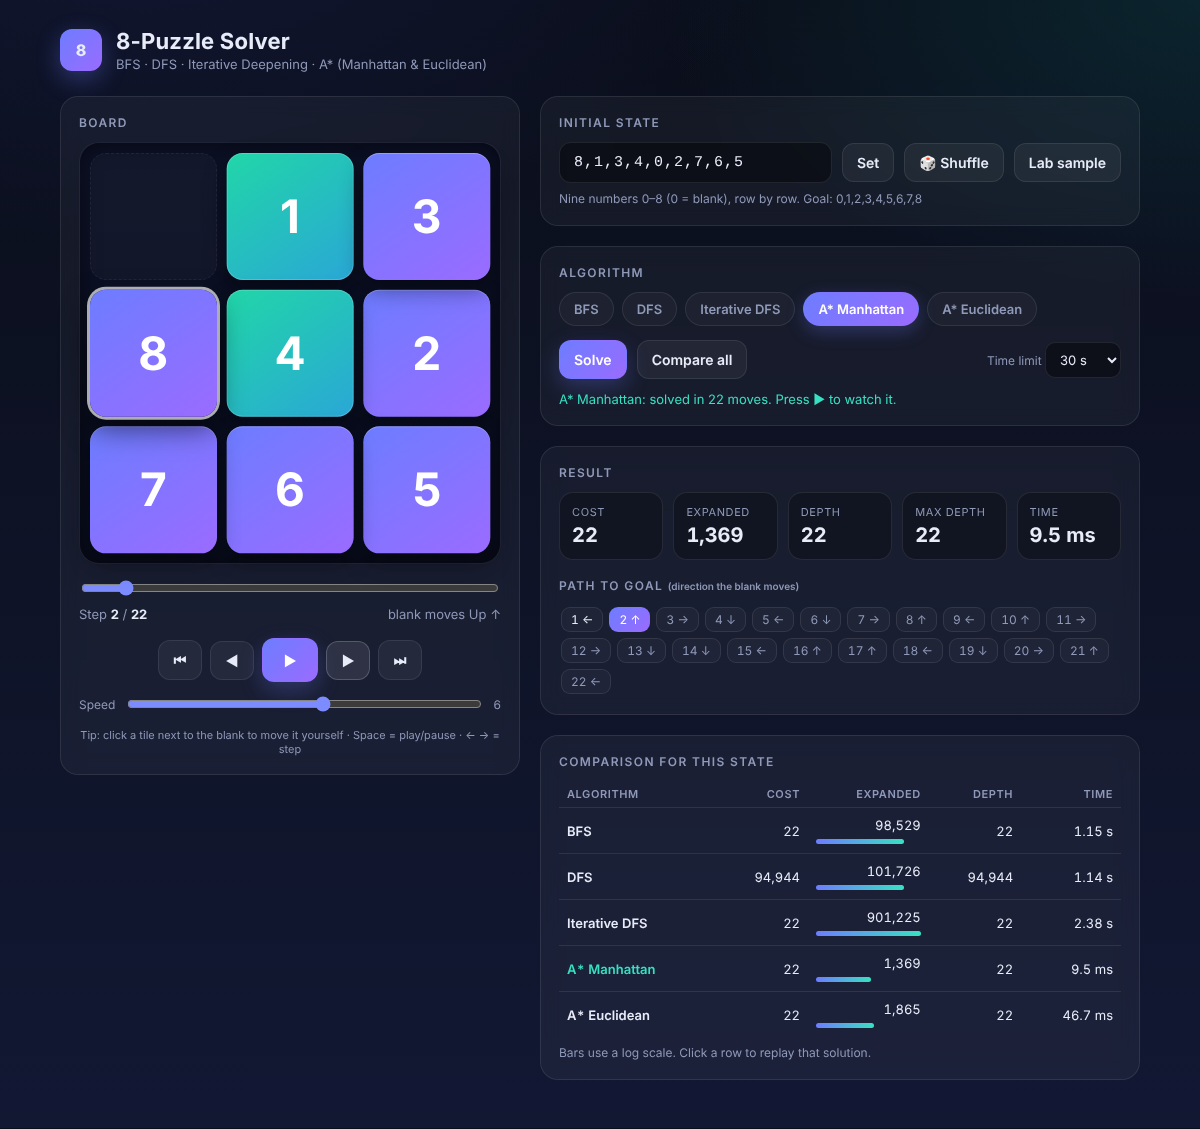
\includegraphics[width=.92\textwidth]{gui.png}\caption{The GUI after ``Compare all'' on \texttt{8,1,3,4,0,2,7,6,5}, replaying the 22-move A* Manhattan solution.}\end{figure}

\section{How to run}
\begin{lstlisting}[language=bash]
python main.py --state 1,2,5,3,4,0,6,7,8 --algo all       # all algorithms, boards printed
python main.py --random --seed 7 --algo all --no-trace    # table only (IDS takes ~30 s)
python main.py --gui                                      # graphical interface
python -m pytest -q                                       # tests
\end{lstlisting}
\end{document}
